% 
%  chapter4.tex
%  ISELthesis
%  
%  Created by Matilde Pós-de-Mina Pato on 2012/10/09.
%
\chapter{Implementation}
\label{cha:impl}

This chapter describes how the architecture and resolution cascade introduced in
Chapter~\ref{ch:proposed_solution} are realised in code. It follows the same two-part structure
as the contribution itself: the Function Registry and the deployment-time resolution mechanism
shared by both cloud providers, and the AWS Lambda support added to QuickFaaS that the
AWS side resolver and deployer depend on.

The chapter is organised in three sections. Section~\ref{sec:function-registry} presents the
Function Registry itself: its file format, how entries are created and kept up to date, and the
internal behaviour of the two provider resolvers that consult it at deployment time. The
following section, AWS Lambda Support in QuickFaaS, traces the concrete deployment steps that
Level~3 of the cascade triggers on AWS --- work that has no equivalent on the GCP path.
Section~\ref{sec:runtime-invocation} closes the chapter by following a resolved internal call
through to its actual invocation once the workflow has been deployed.

\section{Function Registry}
\label{sec:function-registry}

This work introduces a \textit{Function Registry} to decouple workflow definitions from concrete function endpoints, reducing manual coordination between function deployments and workflow orchestration.

Figure~\ref{fig:omniflow-integration-classes} details the classes that realise the unification inside OmniFlow. Function deployment is abstracted behind the \texttt{InternalFunctionDeployer} interface, following the strategy pattern, with three implementations: \texttt{Noop\allowbreak Internal\allowbreak Function\allowbreak Deployer} (the safe default, which raises if invoked), \texttt{QuickFaasDeployer} (GCP), and \texttt{AwsLambdaDeployer} (AWS, added in this work). Each provider deployer (\texttt{Google-\linebreak[4]CloudDeployer}, \texttt{AmazonCloudDeployer}) owns a provider-specific resolver, and both resolvers share two collaborators: the \texttt{FunctionRegistryStore}, which persists bindings as \texttt{FunctionInvocationMetadata} (\texttt{serviceName} plus \texttt{url}, where \texttt{url} is an HTTPS endpoint on GCP and a Lambda ARN on AWS), and the deployer strategy. The \texttt{Function\allowbreak Registry\allowbreak Bootstrapper} populates a missing registry by discovery. This structure keeps the two providers symmetric and makes the deployer a clean extension point: supporting a further platform means adding one resolver and one \texttt{InternalFunctionDeployer}, without touching the existing ones.
\begin{figure}[htbp]
  \centering
  
\includegraphics[width=\textwidth]{images/implementation/omniflow-integration-classes.png}
  \caption{Class model of the integration layer added to OmniFlow.}
  \label{fig:omniflow-integration-classes}
\end{figure}


\subsection{Motivation}
In the original OmniFlow usage model, a \texttt{call} step requires concrete endpoint information (namely \texttt{host} and \texttt{path}). This makes workflows brittle: if a function is redeployed and its endpoint changes, the workflow definition must also be updated. The Function Registry addresses this problem: workflows reference internal functions through stable logical identifiers instead of concrete endpoints. The actual endpoint is only bound to that identifier at deployment time. Beyond endpoint indirection, the registry also serves as the persistence layer for the
automatic function resolution mechanism described below: entries are created and refreshed
automatically as functions are discovered on the target provider or deployed through QuickFaaS.



\subsection{Concept and Conventions}
Each internal function is identified by a stable logical identifier, referred to as
\texttt{functionRef} (e.g., \texttt{"fraud-check"}). Instead of embedding the real endpoint
in the workflow definition, an internal call declares the function through a dedicated DSL
construct, \texttt{internalFunction(name, deploymentDescriptorPath)}, added to the
\texttt{call} step in this work. The two construction paths are mutually exclusive and
enforced at build time:

\begin{itemize}
    \item \textbf{External calls} provide literal \texttt{host} and \texttt{path} values,
    exactly as in the original OmniFlow design, and bypass the registry entirely.
    \item \textbf{Internal calls} provide \texttt{internalFunction(...)} and \emph{must not}
    set \texttt{host} or \texttt{path}: both fields are filled in automatically at deployment
    time from the registry. The optional second argument points to a QuickFaaS deployment
    descriptor, used only when the function cannot be resolved or discovered (see below).
\end{itemize}

For example, an internal function call is declared as:

\begin{lstlisting}[language=Kotlin,caption={Internal call declared with \texttt{internalFunction}},label={lst:internal-call-registry}]
call {
    method(GET)
    internalFunction(
        "fraud-check",
        deploymentDescriptorPath = "./functions/fraud-check/func-deployment.json"
    )
    result("fraudResult")
}
\end{lstlisting}

External calls are unaffected by this mechanism, they continue using literal \texttt{host} and \texttt{path} values and bypass the registry resolution.

\subsection{Registry File Format}
Each provider has its own registry, stored as a JSON file (\texttt{function-registry.gcp.json} or \texttt{function-registry.aws.json} in the working directory by default) and containing only non-secret invocation metadata. It maps each \texttt{functionRef} to the concrete values required to invoke the function (serviceName and url, where url is an HTTPS endpoint on GCP and a Lambda ARN on AWS). The registry also stores an \texttt{updatedAt} timestamp for traceability. Listing~\ref{lst:function-registry} shows a GCP registry holding a function deployed by QuickFaaS (a first-generation Cloud Function) and a Cloud Run service found by discovery under a region-qualified key; an AWS registry has the same structure, with Lambda ARNs as \texttt{url} values.

\begin{lstlisting}[language=json,caption={Function registry structure (GCP)},label={lst:function-registry},basicstyle=\ttfamily\footnotesize]
{
  "updatedAt": "2026-02-15T00:00:00Z",
  "functions": {
    "fraud-check": {
      "serviceName": "fraud-check",
      "url": "https://europe-west1-proj.cloudfunctions.net/fraud-check"
    },
    "europe-west1/risk-score": {
      "serviceName": "projects/proj/locations/europe-west1/services/risk-score",
      "url": "https://risk-score-def456-ew.a.run.app"
    }
  }
}
\end{lstlisting}

\subsection{Creation, Bootstrap and Updates}
The registry management layer provides the following behavior:

\begin{itemize}
    \item \textbf{Bootstrap by discovery:} if the registry file does not exist, it is created
    automatically by listing the functions already deployed on the target provider --- Cloud Run
    services on GCP, Lambda functions on AWS --- and writing one entry per discovered function; on
    AWS this scans every region enabled for the account and, mirroring the GCP catalog, promotes a
    function name seen in more than one region from a bare key to a \texttt{"region/name"} key for
    each occurrence.
    \item \textbf{Automatic registration:} when an internal function is not present in the
    registry but is found on the target provider (Cloud Run service on GCP, Lambda function
    on AWS), a new entry is written immediately with the discovered metadata.
    \item \textbf{Post-deployment updates:} after a successful QuickFaaS deployment, the
    resulting invocation metadata is written to the registry, so subsequent deployments
    resolve the function without redeploying it.
    \item \textbf{Drift handling:} on every registry hit, the stored endpoint is validated
    against the live resource (Cloud Run service on GCP, Lambda function on AWS); if it
    changed, the entry is refreshed, and if the resource no longer exists, the stale entry is
    removed and deployment fails with an explicit diagnostic. First-generation Cloud Functions
    on GCP are not validated (see the limitation at the end of Section~\ref{subsec:store-internals}).
\end{itemize}

Every write refreshes the top-level \texttt{updatedAt} timestamp.

\subsection{Deployment-Time Endpoint Resolution}
\label{subsec:endpoint-resolution}
The registry is consumed at deployment time by an endpoint resolution step. Before rendering the provider-specific workflow artifact (e.g., Google Workflows YAML), OmniFlow inspects each \texttt{CallContext}:
\begin{enumerate}
\item OmniFlow traverses the workflow tree (including nested branches, iterations and
parallel blocks) and intercepts every \texttt{CallContext} carrying an
\texttt{internalFunction} declaration, external calls are left untouched.
\item The registry is consulted for the \texttt{functionRef} (exact match first, then
suffix match on \texttt{"region/functionRef"}). On a hit, the stored URL is used ---
after validating it against the live service (a Cloud Run lookup on GCP, a Lambda
\texttt{GetFunction} call on AWS). If validation detects drift (e.g., a changed ARN)
the registry entry is updated accordingly. If the target no longer exists where the entry
says, the function is searched for in the other regions: if it is found there, the entry is
replaced; otherwise the stale entry is removed and deployment aborts, even when the call
declares a \texttt{deploymentDescriptorPath}. The function existed and was removed, possibly
on purpose, so redeploying it automatically could undo a deliberate deletion; the diagnostic
asks the developer to redeploy the function or update the workflow instead.
\item On a registry miss, the target provider is queried
directly (Cloud Run service lookup across regions on GCP; on AWS, a
\texttt{GetFunction} lookup across every region enabled for the account, or a single
call when the fully-qualified form is used). If the function exists, its metadata is
registered and used and no deployment is triggered.
\item Only if the function is absent from both the registry and the provider, and a
\texttt{deploymentDescriptorPath} was declared, is QuickFaaS invoked to deploy the
function; the returned metadata is registered and used. Otherwise, deployment fails
fast with a diagnostic identifying the unresolved function.
\end{enumerate}
The resolved URL is finally split into \texttt{host} and \texttt{path} (on AWS, into a
\texttt{lambda://<arn>} reference consumed by the renderer) and injected into the call step
before the provider-specific workflow artifact is rendered.
\subsection{Registry Store and Resolver Internals}
\label{subsec:store-internals}

The registry file is manipulated exclusively through \texttt{FunctionRegistryStore}, which
exposes a small, deliberately narrow interface: \texttt{readAll()} parses the whole file into an
ordered map of \texttt{functionRef} to \texttt{FunctionInvocationMetadata}; \texttt{tryResolveEntry()}
re-reads the file via \texttt{readAll()} and delegates the two-step lookup (exact match on
\texttt{functionRef}, then suffix match on \texttt{"region/functionRef"}, raising if the suffix
match is ambiguous) entirely to its pure counterpart, \texttt{tryResolveEntryIn()}, which performs
that lookup against an already-loaded map with no I/O of its own --- the same split
\texttt{resolveUrl()}/\texttt{resolveUrlIn()} already had; \texttt{put()} inserts or refreshes one entry; and
\texttt{remove()} deletes a stale entry. Every mutating operation rewrites the top-level
\texttt{updatedAt} timestamp. The store itself keeps no in-memory state between calls, so
\texttt{readAll()}/\texttt{tryResolveEntry()} re-read and re-parse the file on every call; the
performance consequences of this choice, and the single-read mitigation built on
\texttt{tryResolveEntryIn()}, are analysed in Chapter~\ref{cha:evaluation}.

The two provider resolvers sit on top of this store and are now symmetric in shape, differing only
in the provider-discovery calls that reflect the two clouds' invocation models. \\
\texttt{WorkflowInternalFunctionResolver} (GCP) treats a registry hit as provisional: it
validates the stored URL against the live Cloud Run service and, if the URL has drifted, refreshes
the entry; if the service has disappeared, it attempts rediscovery across the project's regions
and, failing that, removes the stale entry and aborts. It also short-circuits validation for
first-generation Cloud Functions (identified by a \texttt{cloudfunctions.net} URL), which are not
Cloud Run services. When a function is absent from the registry, it is looked up across regions,
and a match in more than one region is reported as ambiguous.\\
\texttt{Aws\allowbreak Internal\allowbreak Function\allowbreak Resolver} follows the same shape: it treats a registry hit
as provisional, resolving the region to validate from the stored ARN and consulting the Lambda API
through a \texttt{Lambda\allowbreak Function\allowbreak Inspector} seam; a drifted ARN refreshes the entry, and a
permissions failure aborts rather than being mistaken for an absence. The resolver mirrors the GCP path and attempts
rediscovery, searching every region enabled for the account before removing the stale entry and
aborting. \\
Region discovery is itself provider-specific: GCP already exposed a project-scoped
locations API, whereas AWS has no equivalent for Lambda, so a dedicated
\texttt{Ec2Aws\allowbreak Regions\allowbreak Lister}, backed by the EC2 \texttt{DescribeRegions} call, was added to
play that role; an optional preferred region, when supplied, is tried first in both the
rediscovery and the miss-path scan described next. \\
On a registry miss, the AWS resolver performs
the same style of scan as GCP: it searches every enabled region for a function-name match,
disambiguating a name found in more than one region, unless the caller supplies the
fully-qualified \texttt{"<region> /<functionRef>"} form, which resolves a single region directly. A
region reporting \texttt{ResourceNotFoundException} and one reporting a permissions failure are
both simply excluded from the candidate set while the scan runs, but the two are told apart at the
end, exactly as on the GCP path: if the function is found in no region and at least one of the
scanned regions was inaccessible, the resolver raises a diagnostic naming those regions instead of
concluding the function is absent everywhere; the absence conclusion is only drawn when every
scanned region reported a clean \texttt{NotFound}. This closes the asymmetry the miss path used to
have, where a single \texttt{GetFunction} call collapsed a genuine absence and a permissions
failure into the same outcome (see \S\ref{subsec:validation-error-semantics}). What now
distinguishes the two resolvers is only the underlying provider API each one calls --- the Cloud
Run Locations API versus EC2 \texttt{DescribeRegions} for region discovery, a Cloud Run lookup
versus \texttt{GetFunction} for the per-region check --- and the GCP-only short-circuit for
first-generation Cloud Functions noted above, which has no AWS counterpart. In both resolvers, a hit or a
successful discovery writes the metadata back through \texttt{put()} before the endpoint is
injected into the call, so the registry converges toward a complete set of bindings as workflows
are deployed.

To keep resolution cheap when a workflow contains many internal calls, both provider resolvers
read the registry once into a snapshot at the start of \texttt{resolve()} and resolve every call
against that in-memory map, keeping it in sync with every subsequent \texttt{put()}/\texttt{remove()}
so that two calls to the same function within one workflow still observe each other's writes,
rather than re-reading the file per call.

\paragraph{Limitation: first-generation Cloud Functions on GCP.}
On GCP, QuickFaaS deploys first-generation Cloud Functions (Section~\ref{sec:background_quickfaas}),
but the GCP resolver's live validation, its provider discovery and the registry bootstrap all query
the Cloud Run API. The functions that the integration itself deploys on GCP are therefore only
partly covered by the cascade. First, a registry hit on a \texttt{cloudfunctions.net} URL is
returned without a live check, so a function that was deleted or moved is not detected at
deployment time: the workflow is deployed against the stored URL, and the failure only surfaces
when the workflow invokes the function. Second, neither the bootstrap nor discovery lists
first-generation functions, so a binding missing from the registry (for example, because the
registry file was deleted or the deployment runs on another machine) cannot be rediscovered. With a
descriptor, the cascade reaches Level~3 and invokes QuickFaaS again for a function that already
exists; without one, deployment fails and reports the function as absent. The AWS path is not
affected. Closing the gap requires a Cloud Functions~v1 client, used for validation, discovery and
bootstrap alongside the Cloud Run one; this is listed as future work (Section~\ref{sec:concl-future}).

\subsection{Resolution Cascade Sequences}
\label{subsec:cascade-sequences}

The description of the two resolvers above is expanded into six sequence diagrams, one per
cascade level and provider, making explicit the messages exchanged with the registry and with
each provider's inspection API; to keep this chapter's flow uninterrupted, the diagrams themselves
are collected in Appendix~\ref{app:cascade-sequences} rather than placed inline.

Figure~\ref{fig:resolution-cascade-level1} (Appendix~\ref{app:cascade-sequences}) details Level~1
on each provider: a registry hit is validated against the live resource before being trusted. The
two panels now show matching behaviour on a \texttt{NotFound} result --- both the GCP path (a) and
the AWS path (b) attempt rediscovery across every region before removing the stale entry and
aborting.

Figure~\ref{fig:resolution-cascade-level2} (Appendix~\ref{app:cascade-sequences}) details Level~2,
reached on a registry miss. Both resolvers now search across every region --- the GCP path (a)
across the project's regions, the AWS path (b) across every region enabled for the account,
discovered via EC2 \texttt{DescribeRegions} --- or a single region when the fully-qualified
\texttt{"region/function- Ref"} form is used, reporting more than one match as ambiguous. On both
paths, a per-region permissions failure is not distinguished from a genuine absence in that region
while at least one other region remains reachable, but if no match is found anywhere and at least
one region was inaccessible, the resolver reports the inaccessible regions explicitly rather than
treating the miss as a plain absence (\S\ref{subsec:validation-error-semantics}).

Figure~\ref{fig:resolution-cascade-level3} (Appendix~\ref{app:cascade-sequences}) details Level~3,
reached only when a \texttt{deployment\allowbreak Descripto-\allowbreak rPath} was supplied and the function was found on
neither the registry nor the provider. Both panels stay at the cascade's conceptual level; the
full operational breakdown of the AWS branch --- the IAM role, the region derived from the S3
bucket, subprocess retries, and \texttt{GetFunction} polling --- is traced separately for the
worst-case path in Figure~\ref{fig:aws-deploy-sequence}, introduced in the AWS Lambda Support
section that follows.

\subsection{Validation and Error Semantics}
\label{subsec:validation-error-semantics}
Several correctness constraints are enforced to avoid silent misconfiguration:

\paragraph{Unresolvable function.}
If a function is absent from the registry and from the target provider, and no deployment
descriptor was provided, deployment fails fast with a message identifying the function and
the corrective actions (deploy it first, or provide \texttt{deploymentDescriptorPath}).

\paragraph{Ambiguous references.}
If a suffix match yields multiple regional entries in the registry, or a function name
exists in multiple regions on the provider, deployment fails with a message instructing the
developer to disambiguate using the fully-qualified form
\texttt{internalFunction("<region>/<functionRef>")}. Unlike an unresolvable function, this
failure is not rescued by supplying a \texttt{deploymentDescriptorPath}: ambiguity is a
data-consistency problem, not an absence one, so QuickFaaS is never invoked to paper over it.

\paragraph{Stale registry entries.}
If a registry entry points to a resource that no longer exists --- a Cloud Run service on GCP, or
a Lambda on AWS, for which rediscovery across every region also fails --- the stale entry is
removed and deployment aborts with an explicit diagnostic, preventing the workflow from being
deployed against a dead endpoint.

\paragraph{Insufficient permissions.}
If the live lookup used to validate a registry hit is refused (an authorization failure rather
than an absence), deployment aborts immediately with a diagnostic naming the function; on GCP no
rediscovery is attempted, since a permissions failure gives no information about whether the
service still exists. The same rule now applies on AWS, where a refused \texttt{GetFunction} is
likewise distinguished from a genuine absence. The distinction is drawn more coarsely on the
miss-path region scan, on both providers: while the scan is running, a region where the lookup is
refused is simply excluded from the candidate set, the same as a region where the function is
absent, so a permissions gap in one region does not by itself stop a match found elsewhere; but if
the scan ends with no match anywhere and at least one region could not be checked, it surfaces a
diagnostic naming the inaccessible regions instead of silently concluding the function is absent
everywhere (see \S\ref{subsec:store-internals}).

\subsection{Registry Location}
The registry file is stored in a writable location at runtime (e.g., the working directory or a configurable path provided to the deployer). This avoids attempting to write into packaged resources (which are typically read-only in production).

\subsection{Evolution of the Registry Design}
\label{subsec:registry-evolution}

The registry did not arrive at its current form in a single step; the source tree still exposes
the intermediate stages, which makes the design decisions worth recounting. Five threads describe
how it evolved.

\paragraph{From literal endpoints to logical indirection.}
The starting point was the plain OmniFlow \texttt{call} step, which embeds a concrete
\texttt{host}/\texttt{path}. This couples the workflow definition to a specific deployed instance
of a function, so any redeployment that changes the endpoint forces an edit to the workflow. The
first design move was therefore to introduce a level of indirection: the workflow names a function
through a stable \texttt{functionRef}, and the concrete endpoint is bound from the registry at
deployment time. The registry exists precisely to hold that binding.

\paragraph{A metadata record per function.}
Each function is represented in the registry by a single structured record,
\texttt{FunctionInvocationMetadata} (a \texttt{serviceName} plus a \texttt{url}), which the two
production resolvers, \texttt{Aws\allowbreak Internal\allowbreak Function\allowbreak Resolver} and
\texttt{Workflow\allowbreak Internal\allowbreak Function\allowbreak Resolver}, consume directly.
Both resolvers read the registry once into an in-memory snapshot per \texttt{resolve()} call and
resolve every internal call against that snapshot, kept in sync with every subsequent
\texttt{put()}/\texttt{remove()}, instead of re-reading the file per call
(Section~\ref{sec:eval-real-resolvers}). The same single-read strategy, isolated from any
cloud-side validation, is also implemented by a benchmark fixture,
\texttt{OptimizedEndpointResolver}, which the local-resolution benchmark suite uses as a pure,
provider-agnostic reference implementation, deliberately decoupled from the live-validation step
the real resolvers must perform against a cloud API.

\paragraph{From provider-specific fields to a uniform endpoint.}
Collapsing the endpoint into one \texttt{url} field was the change that made the AWS extension
cheap. Because \texttt{url} is treated as an opaque, provider-interpreted string --- an HTTPS
endpoint on GCP, a Lambda ARN on AWS --- the registry schema did not have to change when the AWS
provider was added; only the resolver that reads the field and the renderer that consumes it are
provider-aware. The registry thus stayed a single, symmetric abstraction across the two clouds.

\paragraph{From a manually edited file to an auto-managed source of truth.}
The registry also evolved from something the developer would maintain by hand into something the
integration maintains automatically. It is bootstrapped by discovery when absent, populated on the
fly when a function is found on the provider, refreshed after a QuickFaaS deployment, corrected when
a stored URL has drifted, and pruned when an entry becomes stale --- with every write stamping the
top-level \texttt{updatedAt} field. In parallel, the resolution path itself was refined from
re-reading the whole file on every lookup (\texttt{resolveUrl}) toward reading it once into a
snapshot and resolving in memory (\texttt{readAll} + \texttt{resolveUrlIn}); the performance effect
of that refinement, and its propagation into the two production resolvers, are quantified in
Chapter~\ref{cha:evaluation}.

\paragraph{From a trusted cache to a verified indirection.}
The two production resolvers did not always treat a registry hit the same way.
\texttt{Workflow\allowbreak Internal\allowbreak Function\allowbreak Resolver} (GCP) validated every hit against the live
Cloud Run service from the start, because a Cloud Run lookup needs the project/region/service
triple that only the registry supplies. \texttt{Aws\allowbreak Internal\allowbreak Function\allowbreak Resolver} initially
trusted a hit outright, returning the cached ARN with no live check, since a Lambda name is
already unique within a region and validating brought no discovery benefit on its own. This
asymmetry was closed by introducing \texttt{Lambda\allowbreak Function\allowbreak Inspector}, the AWS counterpart to
the Cloud Run inspector: a hit is now confirmed against \texttt{GetFunction} on both providers,
refreshing a drifted ARN and removing a deleted one. The change did not make the registry
redundant, only its trust model stricter: the live check answers whether a binding the registry
already named is still accurate, not what to look up or whether a deployment is owed. Indirection
and idempotency --- the two properties that motivated the registry in the first place
(\S\ref{sec:resolution-cascade}) --- are unaffected by whether the hit is trusted or verified.

\subsection{Summary}
The Function Registry introduces a stable indirection layer between workflow definitions and deployed function endpoints. Internal workflow calls declare a logical \texttt{functionRef} through the
\texttt{internalFunction} DSL construct, and concrete endpoint binding is performed at
deployment time through a resolution cascade (registry, provider discovery, QuickFaaS
deployment as a last resort). This improves maintainability, supports repeatable deployments, and provides explicit, fail-fast diagnostics when registry bindings are missing or inconsistent.

\section{AWS Lambda Support in QuickFaaS}
Figure~\ref{fig:aws-deploy-sequence} traces the end-to-end deployment for the most demanding path, where an internal function exists in neither the registry nor AWS. The three \texttt{alt} fragments correspond directly to the three levels of the resolution cascade described in Section~\ref{subsec:endpoint-resolution}. Once Level~3 is reached, \texttt{AwsLambdaDeployer} performs the AWS-specific work that has no GCP equivalent: it resolves or creates the Lambda execution IAM role, patches the resolved role ARN into a temporary copy of the descriptor, determines the effective region from the S3 bucket's location, and invokes QuickFaaS as a subprocess — retrying up to three times with a 20~s back-off to absorb IAM eventual consistency. After the subprocess returns, it polls \texttt{GetFunction} until the function reaches the \texttt{Active} state (bounded by a 180~s timeout), retrieves the ARN, and grants the Step Functions service permission to invoke the function. The ARN is stored in the registry and, once all calls are resolved, the workflow is rendered with a \texttt{lambda:invoke} task resource and submitted via \texttt{CreateStateMachine}. This diagram makes explicit the operational steps that the conceptual cascade abstracts away. The rationale for invoking QuickFaaS as a subprocess, rather than integrating the two tools as separate communicating services, is discussed in Section~\ref{sec:design-rationale}.

\begin{figure}[htbp]
  \centering
  
\includegraphics[width=\textwidth]{images/implementation/aws-deploy-sequence.png}
  \caption{Deployment sequence on AWS for the worst-case path (function absent from
  both the registry and the provider).}
  \label{fig:aws-deploy-sequence}
\end{figure}

AWS support is realised in two layers that meet at the subprocess boundary: the AWS provider added
\emph{inside} QuickFaaS, which performs the actual Lambda deployment, and the
\texttt{AwsLambdaDeployer} added \emph{inside} OmniFlow, which prepares the environment,
drives QuickFaaS, and produces the invocation metadata the registry stores.

\subsection{The QuickFaaS AWS Provider}
\label{subsec:quickfaas-aws-provider}

The AWS provider extends QuickFaaS's existing abstractions (\texttt{CloudProvider},
\texttt{Cloud\allowbreak Function}, \texttt{CloudRequests}) so that a cloud-agnostic function can be packaged
and deployed to AWS Lambda through the same ZIP strategy used for GCP and Azure. Its core is
\texttt{AwsLambdaFunction.deployZip}, which: uploads the packaged archive to the S3 bucket named in
the descriptor; checks whether the function already exists (\texttt{GetFunction}); and then either
creates it (\texttt{CreateFunction}, with the code referenced as an S3 object) or updates its code
(\texttt{UpdateFunctionCode}), in both cases blocking on the AWS SDK waiter until the function is
active. The handler is fixed to the provider-agnostic entry point \texttt{AwsHttpTemplate}, which
adapts the Lambda request to the developer's hook, and the supported runtimes are \texttt{java11}
and \texttt{java17}. Because \texttt{GetBucketLocation} must be issued against the global endpoint,
the provider resolves the bucket's region from \texttt{us-east-1} and then pins the Lambda client
to that same region, ensuring the function and its code bucket are co-located. Finally, the
provider creates (or reuses) a Lambda \emph{Function URL} with \texttt{AuthType = AWS\_IAM}. This
Function URL is QuickFaaS's own notion of an invocation endpoint; as explained below, the OmniFlow
integration does not use it, preferring the function ARN.

\subsection{The OmniFlow-Side Deployer}
\label{subsec:omniflow-aws-deployer}

\texttt{AwsLambdaDeployer} is the AWS implementation of the \texttt{InternalFunctionDeployer}
strategy. It performs the work that has no GCP equivalent and that must happen \emph{around} the
QuickFaaS subprocess. From the raw descriptor it resolves or creates the Lambda execution IAM role:
if \texttt{iamRoleArn} is blank or a placeholder, it creates a managed
\texttt{OmniFlowLambdaExecutionRole} (attaching \texttt{AWSLambdaBasicExecutionRole}); if a real ARN
is supplied, it verifies and, if necessary, repairs the role's trust policy so that
\texttt{lambda.amazonaws.com} can assume it. The resolved ARN is patched into a temporary copy of
the descriptor, the effective region is taken from the S3 bucket's location, and QuickFaaS is
invoked as a subprocess --- retried up to three times with a 20-second back-off to absorb IAM
eventual consistency. After the subprocess returns, the deployer polls \texttt{GetFunction} until
the function reports the \texttt{Active} state (bounded by a 180-second timeout), retrieves the ARN,
and grants the Step Functions service principal permission to invoke the function.

A deliberate design choice is visible here: although the QuickFaaS provider produces a Function URL,
the OmniFlow deployer discards it and stores the \emph{ARN} in the registry, because internal calls
are rendered with the native \texttt{lambda:invoke} integration (Section~\ref{sec:runtime-invocation})
rather than as HTTP calls to a Function URL. Listing~\ref{lst:aws-descriptor} shows a minimal AWS
deployment descriptor: it differs from the GCP descriptor of
Listing~\ref{lst:quickfaas_json_config} mainly in \texttt{cloudProvider}, the S3 \texttt{bucket},
the Lambda \texttt{runtime}, and the \texttt{iamRoleArn} field (which may be left as a placeholder to
request automatic role creation).

\begin{lstlisting}[language=json,caption={Minimal AWS deployment descriptor for an internal function.},label={lst:aws-descriptor}]
{
  "cloudProvider": "aws",
  "project": "123456789012",
  "iamRoleArn": "<auto>",
  "function": {
    "name": "hello-lambda-fn",
    "location": "eu-west-1",
    "bucket": "run-sources-tfm2526-eu-west-1",
    "runtime": "java17",
    "trigger": { "type": "http" }
  },
  "functionFile": "./MyFunctionClass.java"
}
\end{lstlisting}

\section{Runtime Invocation}
\label{sec:runtime-invocation}
Figure~\ref{fig:aws-runtime-invocation} shows how an internal function is invoked at runtime, once the workflow is deployed. Unlike external calls — which are rendered as \texttt{apigateway:invoke} HTTP tasks — internal calls use the native \texttt{arn:aws:states:::lambda:invoke} integration, with the ARN fixed at deployment time. Step Functions invokes the Lambda directly with the step's payload; the QuickFaaS template entry point adapts the request and delegates to the developer's hook function, and the response is returned under \texttt{\$.Payload}, from which a \texttt{ResultSelector} extracts the value into the step's result variable. Using the native integration rather than an HTTP endpoint avoids per-call request signing and keeps the invocation within the AWS control plane; this choice is confirmed by the renderer, whose emitted resource for internal calls is \texttt{lambda:invoke} (\texttt{AmazonConstantsUtils}).

\begin{figure}[htbp]
  \centering
  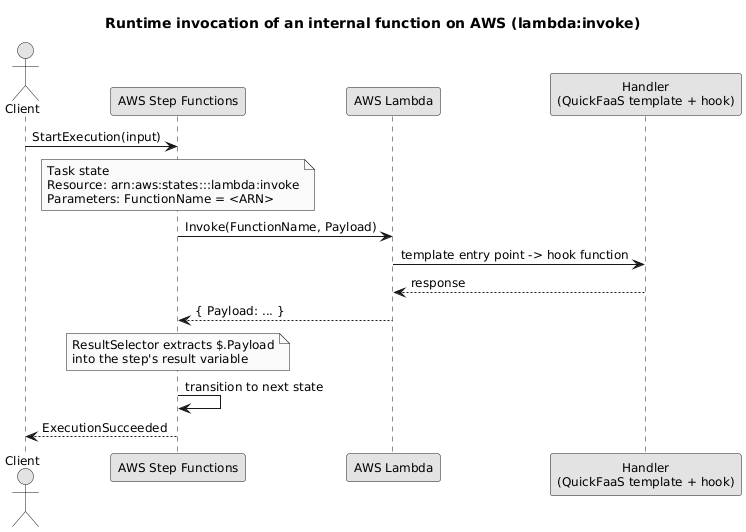
\includegraphics[width=0.8\textwidth]{images/implementation/aws-runtime-invocation.png}
  \caption{Runtime invocation of an internal function on AWS via the native
  \texttt{lambda:invoke} integration.}
  \label{fig:aws-runtime-invocation}
\end{figure}


The distinction between the two forms is made entirely by the renderer,
\texttt{AmazonCall\allowbreak Renderer}, from the \texttt{host} value injected during resolution. If the host
carries the \texttt{lambda://} prefix (the marker written by \texttt{Aws\allowbreak Internal\allowbreak Function\allowbreak Resolver}),
the renderer emits a \texttt{Task} whose \texttt{Resource} is
\texttt{arn:aws:states:::lambda:invoke} and whose \texttt{Parameters} carry the
\texttt{FunctionName} taken from the resolved ARN; any query terms are forwarded under a
\texttt{Payload.queryStringParameters} object. Otherwise it emits the original
\texttt{apigateway:invoke} task with \texttt{ApiEndpoint}, \texttt{Method} and \texttt{Path}. For
the Lambda form the result is extracted with a \texttt{ResultSelector} that reads
\texttt{\$.Payload} into the step's result variable, and the value is scoped under a
\texttt{ResultPath} named after the step so that later steps can reference it. Listing
\ref{lst:rendered-lambda} shows the state a \texttt{call} to \texttt{internalFunction("fraud-check")}
renders to.

\begin{lstlisting}[language=json,caption={Step Functions state rendered for an internal Lambda call.},label={lst:rendered-lambda}]
"fraud-check": {
  "Type": "Task",
  "Resource": "arn:aws:states:::lambda:invoke",
  "InputPath": "$",
  "Parameters": {
    "FunctionName": "arn:aws:lambda:eu-west-1:123456789012:function:fraud-check"
  },
  "ResultSelector": { "fraudResult.$": "$.Payload" },
  "ResultPath": "$.fraud-check",
  "Next": "external-risk-api"
}
\end{lstlisting}

Keeping the internal form as a variant of the existing \texttt{call} renderer --- rather than a new
state type --- means the control-flow, result-passing and error-handling machinery that OmniFlow
already emits for external calls applies unchanged to internal ones; only the \texttt{Resource} and
the parameter shape differ.









































































































































\chapter{Evaluation}
\label{cha:evaluation}

This chapter evaluates the prototype described in Chapter~\ref{cha:impl} and answers the two
research questions of Section~\ref{sec:int_objectives}: whether internal function calls are bound
correctly at deployment time on both providers (RQ1), and how much that resolution costs (RQ2).
Because the contribution of this work is the \emph{unification} layer (the function registry and
the deployment-time resolution cascade) and the AWS provider added to QuickFaaS, the evaluation
concentrates on the decisions the resolution cascade takes, on the cost of resolving
internal-function endpoints and how that cost scales, and on the size overhead of the AWS agnostic
packaging layer.

\section{Scope and Goals}
\label{sec:eval-scope}

Both the correctness checks and the measurements exercise only \emph{local} operations:
constructing a workflow model, traversing it, resolving internal calls against the registry,
reading and writing the registry file, and packaging a Lambda bundle. Operations that call the
cloud provider (Lambda/IAM/S3 requests, Cloud Run/Cloud Functions APIs, the QuickFaaS subprocess)
are deliberately excluded, for two reasons: they are dominated by network and provider-side latency
measured in seconds, and they are non-deterministic and out of the unit-test scope by design. The
correctness checks replace them with test doubles. For RQ2, the evaluation therefore answers a
focused question: \emph{how much does the unification layer add to a deployment, and how does that
overhead scale with the number of calls and the size of the registry?}

The evaluation has four parts:
\begin{itemize}
  \item \textbf{Correctness of the resolution cascade} (RQ1) --- the decision each production
  resolver takes in every situation the cascade can meet, checked by unit tests on both providers.
  \item \textbf{Resolution overhead and scalability} (RQ2) --- the cost of resolving internal calls as a
  function of the number of calls ($N$) and the size of the registry ($R$), and the effect of the
  single-read optimization.
  \item \textbf{Real auto-deploy resolvers} (RQ2) --- the cost of the production resolvers
  (\texttt{Aws\allowbreak Internal\allowbreak Function\allowbreak Resolver}, \texttt{Workflow\allowbreak Internal\allowbreak Function\allowbreak Resolver}) and of the
  registry write path.
  \item \textbf{Packaging overhead} --- the size the AWS provider-agnostic layer adds to a Lambda
  deployment bundle.
\end{itemize}

\section{Correctness of the Resolution Cascade}
\label{sec:eval-correctness}

RQ1 asks whether the resolution cascade binds each internal call to the right endpoint and deploys
a function only when its absence is confirmed. Each production resolver
(\texttt{Aws\allowbreak Internal\allowbreak Function\allowbreak Resolver} and
\texttt{Workflow\allowbreak Internal\allowbreak Function\allowbreak Resolver}) has a unit-test
suite that resolves a small workflow in each situation the cascade can meet. The provider is
replaced by test doubles: a function lookup that answers ``found'', ``not found'' or ``access
denied'' per region, a fixed list of regions, and a deployer that records the deployments it is
asked for. The registry is a real file in a temporary directory. Each test checks the endpoint
written into the call, the registry contents afterwards and, where relevant, whether the deployer
was called or the resolution aborted.

Table~\ref{tab:eval-correctness} lists the situations with the behaviour that the cascade
semantics prescribe (\S\ref{subsec:validation-error-semantics}). The observed behaviour matches the
expected behaviour in every case: all 41 resolver tests (20 for AWS, 21 for GCP) pass, as do the
two tests of the registry bootstrap.

\begin{table}[htbp]
  \centering
  \caption{Situations covered by the resolver unit tests, with the expected behaviour. Each row is
  tested on both AWS and GCP unless marked otherwise; every test passes.}
  \label{tab:eval-correctness}
  \begin{tabular}{p{0.42\textwidth}p{0.48\textwidth}}
    \hline
    \textbf{Situation} & \textbf{Expected and observed behaviour} \\
    \hline
    Registry entry valid (Level~1) & call bound to the registered endpoint \\
    Registry entry whose endpoint changed (drift) & registry updated; call bound to the current
    endpoint \\
    Registry entry for a function no longer in its region (stale) & function searched in all
    regions; if found, the entry is replaced; otherwise the entry is removed and the resolution
    aborts \\
    Validation of a registry entry denied by the provider & resolution aborts; entry kept \\
    Not in the registry, found in one region (Level~2) & call bound; function registered \\
    Found in several regions & resolution aborts (ambiguous name) \\
    Explicit \texttt{region/name} reference & only that region is queried \\
    Every candidate region inaccessible, function not found & resolution aborts with a distinct
    error \\
    Not found anywhere, descriptor given (Level~3) & function deployed once from the descriptor;
    registered; call bound \\
    Not found, some regions inaccessible, descriptor given & resolution aborts; nothing deployed \\
    Internal calls inside branches, iterations and parallel steps & all resolved (five tests) \\
    External calls & host and path unchanged \\
    Several internal calls in one workflow & registry read once \\
    First-generation Cloud Function in the registry (GCP only) & call bound without live
    validation (the limitation of \S\ref{subsec:store-internals}) \\
    Registry file missing (provider-independent) & registry rebuilt from the provider's catalog \\
    \hline
  \end{tabular}
\end{table}

Two situations are not covered by a test: a function that is missing when the call supplies no
deployment descriptor, and a call that sets both \texttt{internalFunction} and a literal
\texttt{host}/\texttt{path}; both resolvers reject either case with an error. Moreover, the tests
check the decisions of the cascade, not the behaviour of the providers: they show that each resolver
acts correctly on what the provider reports, not that the real AWS and GCP APIs report what the
test doubles assume (Section~\ref{sec:eval-threats}).

\section{Methodology}
\label{sec:eval-methodology}

Benchmarks were implemented with the Java Microbenchmark Harness (JMH) 1.37, using
\texttt{AverageTime} mode with results reported in microseconds per operation ($\mu$s/op). Each
measured value is consumed through a \texttt{Blackhole} to prevent dead-code elimination by the
JIT compiler. Unless otherwise stated, runs used one JVM fork with three warm-up iterations and
five measurement iterations of one second each (\texttt{-f 1 -wi 3 -i 5 -w 1 -r 1}), so that the
already-JIT-compiled code is measured. Selected write-path experiments used three forks
(\texttt{-f 3}) to reduce noise.

\paragraph{Caveat on absolute values.}
Measurements were taken on a shared, non-dedicated machine with a deliberately short
configuration. The absolute numbers are therefore meaningful for comparing \emph{trends and
relationships} (linear vs.\ quadratic growth, before vs.\ after an optimization), not as
hardware-definitive figures. Thesis-grade absolute numbers would require repeating the suite with
\texttt{-f 3} on a dedicated machine.

\paragraph{Notation.}
The experiments share five symbols; what changes between them is the \emph{relationship} among
these quantities, summarised in Table~\ref{tab:eval-notation}.

\begin{table}[htbp]
  \centering
  \caption{Notation used throughout the evaluation.}
  \label{tab:eval-notation}
  \begin{tabular}{cl}
    \hline
    \textbf{Symbol} & \textbf{Meaning} \\
    \hline
    $N$ & total number of \texttt{call} steps in the workflow (internal or external), $N = I + E$ \\
    $R$ & number of entries in the registry file when it is read/written \\
    $F$ & number of \emph{distinct} internal functions the workflow references \\
    $I$ & number of internal calls (repetitions counted) \\
    $E$ & number of external calls (repetitions counted) \\
    \hline
  \end{tabular}
\end{table}

$R$ is the physical size of the registry file and is not the same as $F$: a registry may hold
$R{=}1000$ entries while a workflow references only $F{=}10$ of them. Internal calls are
distributed round-robin over the $F$ distinct functions.

\section{Resolution Overhead and Scalability}
\label{sec:eval-resolution}

\paragraph{Cost of the unification.}
The first experiment isolates the cost of resolving an internal call against the cost of an
external call (which bypasses the registry). Resolving an internal call costs about
$7.5\,\mu$s and scales linearly with the number of calls, because each call re-reads and re-parses
the entire registry file from disk; an external call costs about $0.01\,\mu$s
(Table~\ref{tab:eval-p3}). In the general case the cost grows in direct proportion to both the
number of calls and the number of registry entries.

\begin{table}[htbp]
  \centering
  \caption{Resolution cost of internal vs. external calls, with \ $R{=}1$.}
  \label{tab:eval-p3}
  \begin{tabular}{rrr}
    \hline
    \textbf{Calls ($N$)} & \textbf{Internal --- resolved ($\mu$s)} & \textbf{External --- not resolved ($\mu$s)} \\
    \hline
    1   & 7.5    & 0.02 \\
    10  & 74.6   & 0.14 \\
    50  & 368.0  & 0.65 \\
    100 & 747.2  & 1.10 \\
    200 & 1511.4 & 2.34 \\
    \hline
  \end{tabular}
\end{table}

\paragraph{Effect of registry size.}
Fixing the workflow and varying the registry size shows that the per-call cost grows with $R$ and
is essentially independent of $N$: about $180\,\mu$s of fixed I/O and parsing per read plus about
$0.56\,\mu$s per registered entry (Table~\ref{tab:eval-p6}). The four $N$ curves in
Figure~\ref{fig:eval-p6} collapse onto a
single line, confirming that the cost grows in direct proportion to both the number of calls and
the registry size, where the fixed cost of reopening the file dominates for realistic registry
sizes.

\begin{table}[htbp]
  \centering
  \caption{Per-call resolution cost as a function of registry size $R$ (independent of $N$).}
  \label{tab:eval-p6}
  \begin{tabular}{rr}
    \hline
    \textbf{Registry size ($R$)} & \textbf{Cost per call ($\mu$s)} \\
    \hline
    1    & 181.0 \\
    10   & 185.1 \\
    50   & 207.0 \\
    200  & 279.2 \\
    1000 & 741.7 \\
    \hline
  \end{tabular}
\end{table}

\begin{figure}[htbp]
  \centering
  
\includegraphics[width=0.8\textwidth]{images/P6_registry_scaling.png}
  \caption{Per-call resolution cost as a function of registry size $R$, for $N \in \{1, 10, 50,
  200\}$ internal calls; the external-call control does not read the registry.}
  \label{fig:eval-p6}
\end{figure}




\paragraph{The single-read optimization (P7--P9).}
Reading the registry once per workflow into an in-memory snapshot and resolving against it
eliminates that call-times-registry-size product: the cost no longer multiplies the two factors
together, becoming instead one read proportional to the registry size plus a cheap constant-time
lookup per call. Table~\ref{tab:eval-p7} compares, in the same run, resolving
the registry per call (naive) against a single read per resolution (optimized). With the snapshot,
the cost becomes almost independent of $N$, yielding a speedup of up to $\sim$200$\times$ in the
worst corner ($N{=}200$, $R{=}1000$: $\sim$105\,ms down to $\sim$0.54\,ms). Experiments P8 and P9
confirm the same trend on real \texttt{Workflow} objects rather than the isolated store primitive.

\begin{table}[htbp]
  \centering
  \caption{P7 --- total resolution time, naive (per-call read) vs.\ optimized (single read).}
  \label{tab:eval-p7}
  \begin{tabular}{lrrrr}
    \hline
     & $N{=}1$ & $N{=}10$ & $N{=}50$ & $N{=}200$ \\
    \hline
    naive, $R{=}1$       & 4.6   & 47.0   & 233.6   & 920.2    \\
    optimized, $R{=}1$   & 4.7   & 5.0    & 5.0     & 5.7      \\
    naive, $R{=}1000$    & 543.7 & 5480.8 & 26698.5 & 104889.0 \\
    optimized, $R{=}1000$& 557.4 & 535.7  & 551.8   & 536.6    \\
    \hline
  \end{tabular}
\end{table}

\paragraph{Confirming the optimization on real workflows (P8).}
P8 exercises the resolution of a real \texttt{Workflow} object, not the isolated store primitive,
across a grid of $1$ to $50$ distinct functions and $1$ to $200$ calls, with the registry always
hitting ($R{=}F$). The naive path stays dominated by the number of calls and is largely
indifferent to how many distinct functions are involved, at roughly $200\,\mu$s per call at low
$N$ (Table~\ref{tab:eval-p8-naive}), while the optimized path stays close to flat
(Table~\ref{tab:eval-p8-optimized}); the measured speedup climbs from about $1\times$ at $N{=}1$
to about $110\times$ at $N{=}200$.

\begin{table}[htbp]
  \centering
  \caption{P8 --- naive resolution time ($\mu$s) of a real workflow, $F$ distinct functions vs.\
  $N$ calls, $R{=}F$.}
  \label{tab:eval-p8-naive}
  \begin{tabular}{rrrrrr}
    \hline
    $F\backslash N$ & 1 & 5 & 10 & 50 & 200 \\
    \hline
    1  & 216 & 1\,118 & 2\,103 & 9\,544  & 38\,394 \\
    2  & 192 & 956    & 1\,902 & 9\,555  & 37\,950 \\
    5  & 189 & 995    & 1\,911 & 9\,663  & 38\,468 \\
    10 & 195 & 1\,132 & 2\,390 & 10\,544 & 39\,340 \\
    20 & 199 & 997    & 2\,096 & 10\,017 & 41\,205 \\
    50 & 219 & 1\,133 & 2\,194 & 10\,857 & 43\,360 \\
    \hline
  \end{tabular}
\end{table}

\begin{table}[htbp]
  \centering
  \caption{P8 --- optimized (single-read) resolution time ($\mu$s) of a real workflow, same grid
  as Table~\ref{tab:eval-p8-naive}.}
  \label{tab:eval-p8-optimized}
  \begin{tabular}{rrrrrr}
    \hline
    $F\backslash N$ & 1 & 5 & 10 & 50 & 200 \\
    \hline
    1  & 191 & 195 & 197 & 228 & 337 \\
    2  & 191 & 193 & 200 & 230 & 341 \\
    5  & 191 & 194 & 209 & 228 & 349 \\
    10 & 228 & 197 & 202 & 241 & 362 \\
    20 & 199 & 202 & 215 & 237 & 349 \\
    50 & 224 & 221 & 223 & 251 & 367 \\
    \hline
  \end{tabular}
\end{table}

On a realistic workflow ($F{=}10$, $N{=}50$ fixed), P9 isolates the effect of the registry size:
the naive cost climbs with $R$ while the optimized cost stays almost flat, so the speedup grows
from $\sim$41$\times$ at $R{=}10$ to $\sim$58$\times$ at $R{=}1000$ (Table~\ref{tab:eval-p9}).

\begin{table}[htbp]
  \centering
  \caption{P9 --- resolution time ($\mu$s) vs.\ registry size $R$, $F{=}10$/$N{=}50$ fixed.}
  \label{tab:eval-p9}
  \begin{tabular}{rrrr}
    \hline
    \textbf{$R$} & \textbf{naive} & \textbf{optimized} & \textbf{speedup} \\
    \hline
    10   & 9\,829  & 237 & 41.4 \\
    50   & 10\,899 & 268 & 40.7 \\
    200  & 14\,964 & 324 & 46.2 \\
    1000 & 43\,245 & 749 & 57.8 \\
    \hline
  \end{tabular}
\end{table}

\section{Real Auto-Deploy Resolvers and Write Path}
\label{sec:eval-real-resolvers}

\paragraph{Production resolvers (P10, P11).}
Experiments P10 and P11 measure the resolvers that actually run during deployment, one per
provider: \texttt{Aws\allowbreak Internal\allowbreak Function\allowbreak Resolver} (Table~\ref{tab:eval-p10}) and
\texttt{Workflow\allowbreak Internal\allowbreak Function\allowbreak Resolver} (Table~\ref{tab:eval-p11}), with the
registry always hitting ($R{=}F$). Both now carry the single-read optimization demonstrated in
P7--P9 (\S\ref{sec:eval-resolution}): each resolver reads the registry once into a snapshot per
\texttt{resolve()} call and looks up every internal call against it
(\texttt{FunctionRegistryStore.tryResolveEntryIn}) instead of re-reading the file per call. The
result is the same shape as the already-optimized reference implementation: cost is dominated by
$N$ and roughly flat in $F$, at magnitudes comparable to P8's optimized path rather than the
naive, call-times-registry-size cost the unoptimized versions of these classes used to pay. The
two providers land in the same broad range (a few tens to a few thousand microseconds depending on
$N$), with no consistent directional gap between them once the registry-read cost is amortized
--- what asymmetry remains is within the run-to-run noise of this evaluation's shared,
non-dedicated machine (\S\ref{sec:eval-methodology}), most visible at $F{=}10,N{=}5$ in
Table~\ref{tab:eval-p10} and $F{=}50,N{=}50$, both flagged by their own unusually wide error
margins rather than reflecting a code effect.

\begin{table}[htbp]
  \centering
  \caption{P10 --- AWS provider: resolution time ($\mu$s) of the real resolver
  (\texttt{Aws\allowbreak Internal\allowbreak Function\allowbreak Resolver}), $R{=}F$, after the
  single-read optimization was propagated into it.}
  \label{tab:eval-p10}
  \begin{tabular}{lrrrrr}
    \hline
    $F\backslash N$ & 1 & 5 & 10 & 50 & 200 \\
    \hline
    1  & 17 & 44  & 124 & 1\,240 & 3\,486 \\
    10 & 19 & 171 & 85  & 424    & 1\,702 \\
    50 & 52 & 48  & 98  & 1\,669 & 1\,889 \\
    \hline
  \end{tabular}
\end{table}

\begin{table}[htbp]
  \centering
  \caption{P11 --- GCP provider: resolution time ($\mu$s) of the real resolver
  (\texttt{Workflow\allowbreak Internal\allowbreak Function\allowbreak Resolver}), $R{=}F$, after
  the single-read optimization was propagated into it.}
  \label{tab:eval-p11}
  \begin{tabular}{lrrrrr}
    \hline
    $F\backslash N$ & 1 & 5 & 10 & 50 & 200 \\
    \hline
    1  & 20 & 47  & 83  & 353 & 1\,417 \\
    10 & 47 & 105 & 213 & 963 & 2\,966 \\
    50 & 31 & 61  & 99  & 402 & 1\,573 \\
    \hline
  \end{tabular}
\end{table}

\paragraph{Registry write path (P13, P17).}
Writing is more expensive than resolving. Every \texttt{put()} re-reads and rewrites the entire
registry file, so writing $K$ functions into a registry that already holds $R_0$ entries takes
longer than linear time in $K$ (Table~\ref{tab:eval-p13}): each successive write pays for a
registry that has grown by one entry since the write before it, so the cost compounds as $K$
grows, on top of the floor set by $R_0$. The miss-then-write pattern the real resolvers perform
before any cloud call (\texttt{tryResolveEntry} followed by \texttt{put}) adds a further
24--54\% on top (Table~\ref{tab:eval-p17}), since \texttt{tryResolveEntry} is itself a
registry-size-proportional scan. In absolute terms these values remain
in the hundreds of microseconds to low hundreds of milliseconds even for $K{=}100$ successive
writes. The $R_0{=}1000$ column in Table~\ref{tab:eval-p13} does not follow the otherwise
monotonic pattern at $K{=}100$; this single data point is attributed to noise on the shared,
non-dedicated benchmarking machine (\S\ref{sec:eval-methodology}), not to a code effect.

\begin{table}[htbp]
  \centering
  \caption{P13 --- total write time ($\mu$s): $K$ successive \texttt{put} calls, initial registry
  size $R_0$.}
  \label{tab:eval-p13}
  \begin{tabular}{lrrrrr}
    \hline
    $K\backslash R_0$ & 0 & 10 & 50 & 200 & 1000 \\
    \hline
    1   & 2\,673   & 2\,860   & 3\,235   & 4\,139   & 2\,761   \\
    10  & 27\,691  & 26\,986  & 29\,912  & 39\,164  & 24\,029  \\
    100 & 329\,757 & 304\,187 & 330\,100 & 419\,531 & 237\,910 \\
    \hline
  \end{tabular}
\end{table}

\begin{table}[htbp]
  \centering
  \caption{P17 --- total write time ($\mu$s): $K$ successive miss+\texttt{put} pairs, initial
  registry size $R_0$.}
  \label{tab:eval-p17}
  \begin{tabular}{lrrrrr}
    \hline
    $K\backslash R_0$ & 0 & 10 & 50 & 200 & 1000 \\
    \hline
    1   & 3\,309   & 3\,545   & 3\,959   & 5\,122   & 4\,243   \\
    10  & 35\,107  & 34\,358  & 37\,190  & 47\,631  & 47\,817  \\
    100 & 410\,389 & 382\,140 & 403\,488 & 511\,878 & 346\,068 \\
    \hline
  \end{tabular}
\end{table}

\section{Match Strategy, Mixed Workflows, and Structure}
\label{sec:eval-secondary}

\paragraph{Exact vs.\ suffix match (P14).}
The suffix-match path (regional disambiguation) fails the exact lookup and scans the loaded map,
reintroducing a cost proportional to the registry size, but over an already-loaded map: the ratio
to exact match grows to only $\sim$1.9$\times$ at $R{=}1000$ and remains cheap in absolute terms
(Table~\ref{tab:eval-p14}).

\begin{table}[htbp]
  \centering
  \caption{P14 --- exact vs.\ suffix match ($\mu$s), $F{=}10$/$N{=}50$ fixed.}
  \label{tab:eval-p14}
  \begin{tabular}{rrrr}
    \hline
    \textbf{$R$} & \textbf{exact} & \textbf{suffix} & \textbf{ratio} \\
    \hline
    10   & 219 & 228   & 1.04 \\
    100  & 259 & 333   & 1.29 \\
    200  & 309 & 442   & 1.43 \\
    1000 & 768 & 1\,456 & 1.90 \\
    \hline
  \end{tabular}
\end{table}

\paragraph{Mixed internal/external workflows (P15, P16).}
The first workflows to mix internal and external calls confirm that resolution cost scales with
$I$ (internal calls), not with $N{=}I{+}E$: the $I{=}0$ line stays flat as $E$ grows to 200,
because external calls incur no registry lookup (Table~\ref{tab:eval-p15}). The registry-size
effect proved in P9 is unchanged, within the same order of magnitude, when a fraction of the
calls are external (Table~\ref{tab:eval-p16}).

\begin{table}[htbp]
  \centering
  \caption{P15 --- resolution time ($\mu$s) of a mixed workflow, $R{=}F{=}10$ fixed;
  $I$ internal vs.\ $E$ external calls.}
  \label{tab:eval-p15}
  \begin{tabular}{rrrrrr}
    \hline
    $I\backslash E$ & 0 & 1 & 10 & 50 & 200 \\
    \hline
    0   & 181 & 190 & 187 & 183 & 183 \\
    10  & 189 & 205 & 203 & 189 & 255 \\
    50  & 217 & 217 & 230 & 219 & 322 \\
    200 & 326 & 321 & 323 & 315 & 393 \\
    \hline
  \end{tabular}
\end{table}

\begin{table}[htbp]
  \centering
  \caption{P16 --- resolution time ($\mu$s) vs.\ registry size $R$, mixed workflow with
  $I{=}40$/$E{=}10$/$F{=}10$ fixed.}
  \label{tab:eval-p16}
  \begin{tabular}{rr}
    \hline
    \textbf{$R$} & \textbf{Time ($\mu$s)} \\
    \hline
    10   & 346 \\
    50   & 247 \\
    200  & 306 \\
    1000 & 776 \\
    \hline
  \end{tabular}
\end{table}

\paragraph{Workflow shape (P18, P19).}
Nesting depth (P18) leaves the time essentially constant ($\sim$200\,$\mu$s across depths 0--5),
and parallel width (P19) grows only with the total number of internal leaf calls
($N = 5\times\text{width}$), in the same order of magnitude as the flat workflows of P8/P15
(Tables~\ref{tab:eval-p18} and~\ref{tab:eval-p19}). Although the resolver recurses explicitly into
\texttt{Iteration} and \texttt{Parallel} contexts, the shape of the tree is irrelevant: only the
count of internal calls matters.

\begin{table}[htbp]
  \centering
  \caption{P18 --- resolution time ($\mu$s) vs.\ nesting depth, 20 internal calls fixed,
  $R{=}F{=}10$.}
  \label{tab:eval-p18}
  \begin{tabular}{rr}
    \hline
    \textbf{Depth} & \textbf{Time ($\mu$s)} \\
    \hline
    0 & 207.3 \\
    2 & 200.7 \\
    3 & 200.4 \\
    5 & 199.6 \\
    \hline
  \end{tabular}
\end{table}

\begin{table}[htbp]
  \centering
  \caption{P19 --- resolution time ($\mu$s) vs.\ \texttt{Parallel} branch width,
  $N = 5\times$ width, $R{=}F{=}10$.}
  \label{tab:eval-p19}
  \begin{tabular}{rrr}
    \hline
    \textbf{Branches} & \textbf{$N$} & \textbf{Time ($\mu$s)} \\
    \hline
    1   & 5   & 188.3 \\
    10  & 50  & 220.8 \\
    20  & 100 & 276.2 \\
    100 & 500 & 583.7 \\
    \hline
  \end{tabular}
\end{table}

\section{Packaging Overhead (S1)}
\label{sec:eval-bundle}

The AWS provider added in this work packages a Lambda through the QuickFaaS agnostic layer (the
developer hook plus the \texttt{AwsHttpTemplate} adapter and \texttt{aws-lambda-java-core}). Table
\ref{tab:eval-s1} compares the resulting bundle against an equivalent native \texttt{RequestHandler}
implementation of the same logic. The agnostic layer adds about $0.9$\,KB --- 6.6\% of a trivial
bundle, and well under 0.1\% of a real function --- consistent with the original QuickFaaS
evaluation for GCP and Azure.

\begin{table}[htbp]
  \centering
  \caption{S1 --- Lambda bundle size, AWS agnostic layer vs.\ native implementation.}
  \label{tab:eval-s1}
  \begin{tabular}{lr}
    \hline
    \textbf{Bundle} & \textbf{Size} \\
    \hline
    AWS agnostic (QuickFaaS hook + \texttt{AwsHttpTemplate} + \texttt{aws-lambda-java-core}) & 14\,552 bytes \\
    AWS native (single \texttt{RequestHandler}, same logic) & 13\,647 bytes \\
    \textbf{Delta (agnostic-layer overhead)} & \textbf{905 bytes} \\
    \hline
  \end{tabular}
\end{table}

\section{Discussion}
\label{sec:eval-discussion}

\paragraph{Answer to RQ1.}
In every situation of Table~\ref{tab:eval-correctness}, both resolvers take the expected decision:
each internal call is bound to the registered, current or discovered endpoint, and a function is
deployed only when it is in neither the registry nor any region and every region could be checked.
Stale entries that cannot be rediscovered, ambiguous names and inaccessible regions abort the
resolution instead of binding a call to a guess or deploying a duplicate. The answer to RQ1 is
therefore positive for the resolution logic on both providers, with two qualifications: the
evidence comes from tests that simulate the provider, and on GCP a binding to a first-generation
Cloud Function is trusted without a live check.

\paragraph{Answer to RQ2.}
For RQ2, the benchmarks support six conclusions.

First, the cost of the unification is small per call and linear, and its scaling is well
characterised: a cost that grows in direct proportion to both the number of calls and the
registry size in the naive form, dominated by the fixed cost of reopening the
registry file until $R \approx 320$. Second, the single-read optimization eliminates that
call-times-registry-size product, reducing resolution to a cost proportional only to the sum of
the number of calls and the registry size, with a $\sim$200$\times$ speedup in the worst case
(P7, P8, P9) --- a full \emph{identify (P3/P6) $\rightarrow$ fix $\rightarrow$ quantify (P7)} loop.
Third, this optimization has since been propagated to the production resolvers (P10, P11), which
now show the same dominated-by-$N$, flat-in-$F$ shape as the optimized reference path rather than
the call-times-registry-size cost they used to pay.
Fourth, the AWS agnostic packaging layer adds negligible size (S1). Fifth, resolution cost tracks
the number of internal calls rather than the workflow's total call count: external calls add only
the shared tree-traversal cost, never a registry lookup (P15, P16). Sixth, neither nesting depth
nor parallel width changes the cost beyond what the total count of internal calls already
predicts: the resolver's explicit recursion into \texttt{Iteration} and \texttt{Parallel} contexts
is free in practice (P18, P19).

\paragraph{Global framing.}
All measured values lie between microseconds and, in the worst non-optimized write case,
a few hundred milliseconds. Endpoint resolution is therefore not the bottleneck of an integrated
deployment: the dominant cost is the actual cloud deployment (seconds). With the single-read
optimization now applied uniformly across both production resolvers, the overhead of the
unification is asymptotically linear and practically irrelevant in real operation.

\section{Threats to Validity}
\label{sec:eval-threats}

The absolute numbers were obtained on a shared machine with a short JMH configuration; some
experiments used a single fork, which widens error margins. The measurements are consistent among
themselves and with the expected asymptotic forms, but should be reproduced with \texttt{-f 3} on
dedicated hardware before being read as definitive. The evaluation is also intentionally
local-only: it quantifies the resolution and packaging overhead, not the end-to-end cloud
deployment latency, which depends on provider-side behaviour outside the scope of this work.

The correctness evidence for RQ1 has a similar limit. The resolver tests replace the provider with
test doubles, so they establish that each resolver takes the right decision given what the provider
reports, not that the real AWS and GCP APIs report what the doubles assume. The two full-deployment
tests that exercise the real providers need cloud credentials and are excluded from the automated
test suite.






























































































\chapter{Case Study: Real-Time Fraud Detection for Card Payments}
\label{cha:case-study}

The previous chapters described the Function Registry and resolution cascade in isolation from
any particular domain (Chapter~\ref{ch:proposed_solution}), traced their implementation
(Chapter~\ref{cha:impl}), and quantified their overhead (Chapter~\ref{cha:evaluation}). This
chapter grounds those mechanisms in a single, illustrative scenario drawn from retail banking:
a card-payment authorization workflow that screens every transaction for fraud before it is
settled. The scenario is not a validated production deployment; it is a realistic composition of
the \texttt{FraudPipeline} example already introduced in Section~\ref{sec:developer-workflow},
extended to internalize both scoring functions and to make an authorization decision, used here
to walk through the integration end to end and to discuss where it fits --- and where it does not
yet fit --- an actual banking environment.

The chapter is organised as follows. Section~\ref{sec:case-scenario} sets out the business
requirements a payment-authorization workflow imposes and why they line up with the problem this
work addresses. Section~\ref{sec:case-design} defines the workflow in the OmniFlow DSL.
Section~\ref{sec:case-deployment} walks the resolution cascade through two deployments of that
same workflow --- first to AWS, then to GCP --- to make the provider-symmetry claim concrete.
Section~\ref{sec:case-runtime} follows a transaction through the deployed workflow at runtime, and
Section~\ref{sec:case-discussion} discusses the scenario's relevance and its limits, connecting
back to the gaps already identified in Chapter~\ref{cha:conclusions}.

\section{Scenario and Requirements}
\label{sec:case-scenario}

Consider a bank that authorizes card payments through a workflow rather than a monolithic
service: each transaction is screened by two independent scoring functions before the bank
decides whether to settle it. \texttt{fraud-check} is a rules/ML-based service that flags
transactions matching known fraud patterns; \texttt{risk-score} computes a numeric risk score from
transaction and account features. Both are internal functions owned by the bank's fraud team,
deployed and iterated on independently of the orchestration logic. A third, external call settles
approved transactions against the bank's core banking system, which is a distinct system with its
own release cycle and is not managed through the registry.

Three requirements are characteristic of this setting and motivate the integration described in
this dissertation:

\begin{itemize}
    \item \textbf{Frequent, independent model updates.} Fraud-detection models are retrained and
    redeployed far more often than the orchestration logic that calls them --- sometimes daily, in
    response to newly observed fraud patterns. If the workflow definition embedded a concrete
    endpoint for \texttt{fraud-check}, every redeployment of the model would risk requiring a
    matching workflow redeployment, exactly the coupling problem motivating the Function Registry
    (Section~\ref{subsec:endpoint-resolution}).
    \item \textbf{Multi-cloud posture.} Operational-resilience regulation applicable to EU banks,
    notably the Digital Operational Resilience Act (DORA), pushes institutions to avoid
    concentration risk on a single cloud provider for critical functions. A fraud-screening
    workflow is a plausible candidate for a documented ability to run on a second provider, which
    requires the orchestration and the functions it calls to be portable, not just the
    infrastructure underneath them.
    \item \textbf{Auditability of bindings.} A bank's change-management process typically requires
    a record of which concrete function version and endpoint served a given deployment, which the
    registry's \texttt{updatedAt}-stamped entries provide in embryonic form
    (Section~\ref{subsec:registry-evolution}), even though a production deployment would need the
    stronger guarantees discussed in Section~\ref{sec:case-discussion}.
\end{itemize}

\section{Workflow Design}
\label{sec:case-design}

Listing~\ref{lst:case-payment-workflow} defines \texttt{PaymentAuthorization}. The first two
steps call \texttt{fraud-check} and \texttt{risk-score} through \texttt{internalFunction}, so
their endpoints are resolved through the registry at deployment time rather than hard-coded, as
described in Section~\ref{subsec:endpoint-resolution}. Unlike the external \texttt{risk-score}
variant shown in Listing~\ref{lst:wf-external-part}, both scoring calls here are internal and
therefore registry-managed --- a distinction to a partner-owned endpoint the bank happens to also
call. Their results are captured in \texttt{fraudResult} and \texttt{riskResult}. A third step,
\texttt{decision}, is a conditional (\texttt{switch}) step: it jumps to
\texttt{decline-transaction} if the fraud check flagged the transaction or the risk score exceeds
a threshold, and otherwise falls through to the \texttt{default}, \texttt{approve-transaction}.
The approve path issues an external call to the bank's own settlement endpoint, declared with a
literal \texttt{host}/\texttt{path} and therefore bypassing the registry entirely, exactly like
\texttt{external-risk-api} in Listing~\ref{lst:wf-external-part}: the settlement system is not a
function this integration deploys or resolves.

\begin{lstlisting}[language=Kotlin,caption={PaymentAuthorization workflow: two internal scoring calls feeding a decision.},label={lst:case-payment-workflow},basicstyle=\ttfamily\small,breaklines=false]
val PaymentAuthorization = workflow {
  name("PaymentAuthorization")
  description(
    "Real-time fraud screening for card payment authorization")
  input("transaction")
  steps(
    step {
      name("fraud-check")
      context(call {
        method(POST)
        internalFunction("fraud-check", "./deploy/fraud-check.json")
        body(variable("transaction"))
        result("fraudResult")
      })
    },
    step {
      name("risk-score")
      context(call {
        method(POST)
        internalFunction("risk-score", "./deploy/risk-score.json")
        body(variable("transaction"))
        result("riskResult")
      })
    },
    step {
      name("decision")
      context(switch {
        conditions(
          condition {
            match(variable("fraudResult.body.flagged")
              equalTo value(true))
            jump("decline-transaction")
          },
          condition {
            match(variable("riskResult.body.score")
              greaterThan value(75))
            jump("decline-transaction")
          }
        )
        default("approve-transaction")
      })
    },
    step {
      name("approve-transaction")
      context(call {
        method(POST)
        host("core-banking.internal.example")
        path("/v1/settlements")
        body(variable("transaction"))
        result("settlementResult")
      })
    },
    step {
      name("decline-transaction")
      context(assign {
        variables(variable("decision") equalTo value("declined"))
      })
    }
  )
  result("decision")
}
\end{lstlisting}

Nothing in Listing~\ref{lst:case-payment-workflow} names a cloud provider, a region or a concrete
endpoint for either scoring function: that information is supplied once, at deployment time,
through the QuickFaaS descriptors referenced by \texttt{internalFunction} and the choice of
provider deployer. This is what makes the same definition deployable to either provider, as
Section~\ref{sec:case-deployment} shows next.

\section{Deploying the Same Workflow to Two Providers}
\label{sec:case-deployment}

Suppose neither \texttt{fraud-check} nor \texttt{risk-score} has been deployed yet, and the bank
deploys \texttt{PaymentAuthorization} to AWS first. OmniFlow bootstraps an AWS registry by
listing Lambda functions across every enabled region, finds it empty for both functions, and the
cascade reaches Level~3 for each: QuickFaaS deploys \texttt{fraud-check} and \texttt{risk-score}
as Lambda functions from the descriptors referenced in the workflow, following the AWS deployment
sequence detailed in Figure~\ref{fig:aws-deploy-sequence} --- IAM role resolution, subprocess
invocation, \texttt{GetFunction} polling and Step Functions invoke permissions. Both ARNs are
written to the registry, and \texttt{PaymentAuthorization} is deployed as a state machine.

A week later, the fraud team retrains and redeploys \texttt{fraud-check} with an updated model,
using QuickFaaS directly against the same \texttt{functionRef}; the redeployment updates the
Lambda's code (\texttt{UpdateFunctionCode}) without changing its ARN, so the registry entry stays
valid. The next time \texttt{PaymentAuthorization} is deployed --- unchanged, from the developer's
point of view --- \texttt{fraud-check} resolves as a Level~1 registry hit and no redeployment is
triggered by the workflow deployment itself; the workflow definition never had to change to pick
up the new model.

Now suppose the bank wants a documented ability to run the same fraud-screening workflow on a
second provider, per the multi-cloud requirement in Section~\ref{sec:case-scenario}. Because
\texttt{PaymentAuthorization} names no provider, deploying it to GCP requires no change to
Listing~\ref{lst:case-payment-workflow} --- only different QuickFaaS descriptors (targeting Cloud
Functions instead of Lambda) and the GCP deployer. On this first GCP deployment, the GCP registry is
bootstrapped separately from the AWS one, both scoring functions miss at Level~1 and Level~2, and
Level~3 deploys them as first-generation Cloud Functions instead, following the ZIP-based
deployment path described in Section~\ref{sec:background_quickfaas}. The two registries stay
independent, one per provider (\texttt{function-registry.aws.json} and
\texttt{function-registry.gcp.json} by default), so the same \texttt{functionRef} resolves to a
Lambda ARN under one deployment and to a Cloud Functions URL under the other. On GCP, however, those
bindings are not validated on later deployments (\S\ref{subsec:store-internals}). The uniform
\texttt{url} field discussed in
Section~\ref{subsec:registry-evolution} is precisely what makes this substitution transparent to
the workflow definition.

\section{Runtime Invocation}
\label{sec:case-runtime}

Once deployed, a transaction flows through \texttt{PaymentAuthorization} differently depending on
which deployment served it, even though the DSL is identical. On the AWS deployment, Step
Functions invokes \texttt{fraud-check} and \texttt{risk-score} through the native
\texttt{arn:aws:states:::lambda:invoke} integration described in Section~\ref{sec:runtime-invocation}
and shown in Figure~\ref{fig:aws-runtime-invocation}, with the ARN fixed at deployment time; the
\texttt{decision} step is rendered as a native \texttt{Choice} state evaluating
\texttt{fraudResult}/\texttt{riskResult}, and \texttt{approve-transaction} is rendered as the
\texttt{apigateway:invoke}-style HTTP task, since its endpoint was declared with a literal
\texttt{host}/\texttt{path} rather than resolved through the registry. On the GCP deployment, the
same two scoring calls are rendered as HTTP calls to the resolved Cloud Functions URLs, since GCP has no
Lambda-style native invoke equivalent in this integration. In both cases, the decision logic and
the settlement call are unaffected by which provider deployed the scoring functions: only the
\texttt{Resource}/\texttt{call} shape the renderer emits for the two internal steps differs, which
is exactly the boundary Section~\ref{sec:runtime-invocation} identified as provider-specific.

\section{Discussion}
\label{sec:case-discussion}

This scenario exercises the integration's central claim in a setting where it plausibly matters:
a bank can retrain and redeploy a fraud model on its own cadence without touching the
orchestration that calls it, and can retarget the same workflow definition at a second cloud
provider by changing deployment descriptors rather than the workflow itself. Both properties speak
directly to the two motivating forces in Section~\ref{sec:case-scenario} --- independent model
lifecycles and a documented multi-provider posture --- without requiring the fraud or platform
teams to hand-maintain endpoint bindings across redeployments.

The scenario equally exposes why this remains illustrative rather than production-ready. The
gaps already identified in Section~\ref{sec:concl-critical} are not hypothetical here: a registry
holding the live endpoint of a bank's fraud-screening function, writable by any deployment process
with filesystem access and carrying no integrity guarantee, is not a control a bank's
change-management or security function would accept as-is, and the AWS path's broad, automatically
granted IAM role is similarly at odds with a least-privilege environment handling payment data.
The applicability discussion in Section~\ref{sec:concl-applicability} and the corresponding future
work in Section~\ref{sec:concl-future} --- a hardened, access-controlled registry backend with an
attributable write history, and least-privilege IAM under change control --- describe exactly the
hardening this scenario would require before the workflow in
Listing~\ref{lst:case-payment-workflow} could authorize real transactions.




























































































\chapter{Conclusions and Future Work}
\label{cha:conclusions}

This dissertation set out to unify two previously independent tools --- QuickFaaS, which deploys
serverless functions, and OmniFlow, which defines and deploys workflows --- so that a serverless
application can be deployed from a single workflow definition, without manually coordinating
function endpoints. This final chapter summarises the contribution, revisits the objectives,
assesses the work critically, and outlines future directions.

\section{Summary of Contributions}
\label{sec:concl-contributions}

The work delivered two complementary halves.

\paragraph{Unification (core).}
OmniFlow was extended with a \emph{Function Registry} and a deployment-time \emph{resolution
cascade}. Internal workflow calls declare a stable logical identifier through the
\texttt{internalFunction(name, deploymentDescriptorPath)} construct added to the \texttt{call}
step, mutually exclusive with the literal \texttt{host}/\texttt{path} of external calls. At
deployment time OmniFlow traverses the workflow tree, and for each internal call resolves the
endpoint from the registry, discovers it directly on the provider, or --- as a last resort ---
deploys it through QuickFaaS, writing the resulting metadata back to the registry. Function
deployment is abstracted behind the \texttt{InternalFunctionDeployer} strategy interface, which
keeps the two providers symmetric and makes support for a further platform a matter of adding one
resolver and one deployer.

\paragraph{AWS support (complement).}
QuickFaaS, previously limited to GCP and Azure, was extended with an AWS provider, and OmniFlow
gained an \texttt{AwsLambdaDeployer} that performs the AWS-specific work (IAM execution role,
region resolution from the S3 bucket, readiness polling, and granting Step Functions permission to
invoke the Lambda). Internal AWS calls are rendered with the native
\texttt{arn:aws:states:::lambda:invoke} integration rather than an HTTP task, keeping the
invocation within the AWS control plane.

\section{Objectives Revisited}
\label{sec:concl-objectives}

The two research questions of Section~\ref{sec:int_objectives} are answered as follows:
\begin{itemize}
  \item \textbf{RQ1 (feasibility and correctness)} --- yes, for the resolution logic. On both AWS
  and GCP the cascade binds each internal call to the right endpoint and deploys a function only
  when its absence is confirmed, and it aborts on stale entries, ambiguous names and inaccessible
  regions (Section~\ref{sec:eval-correctness}). The evidence comes from unit tests that simulate
  the provider, and on GCP bindings to first-generation Cloud Functions are not validated live.
  \item \textbf{RQ2 (overhead)} --- small. In the production resolvers, resolving a workflow with
  up to 200 internal calls takes at most a few milliseconds locally, growing linearly with the
  number of internal calls, while the registry is read once per deployment
  (Section~\ref{sec:eval-discussion}). These figures exclude the provider calls that validation,
  discovery and deployment make.
\end{itemize}

Against the four objectives stated in Section~\ref{sec:int_objectives}, the work stands as
follows:
\begin{enumerate}
  \item \textbf{Design a unified integration architecture} --- \emph{met.} The registry, the
  \texttt{functionRef} indirection, the \texttt{internalFunction} construct and the resolver
  strategy (Chapters~\ref{ch:proposed_solution} and~\ref{cha:impl}) let a single workflow
  definition drive both function and workflow deployment, binding endpoints when the workflow is
  deployed (\S\ref{sec:resolution-cascade}).
  \item \textbf{Implement an orchestration prototype} --- \emph{met on AWS, partially met on GCP.}
  The prototype resolves the internal functions of a workflow on both providers, and deploys the
  missing ones, without endpoints being copied by hand. On GCP, however, the first-generation Cloud
  Functions that QuickFaaS deploys are not covered by validation or discovery: a stale binding to
  one of them goes undetected, and a binding lost from the registry cannot be rediscovered
  (\S\ref{subsec:store-internals}).
  \item \textbf{Extend QuickFaaS to AWS Lambda} --- \emph{met.} QuickFaaS gained an AWS provider
  and OmniFlow an \texttt{AwsLambdaDeployer} (Sections~\ref{subsec:quickfaas-aws-provider}
  and~\ref{subsec:omniflow-aws-deployer}). The provider-agnostic packaging layer adds about
  0.9\,KB to a Lambda bundle (Table~\ref{tab:eval-s1}), and the resolver tests cover both
  providers (Section~\ref{sec:eval-correctness}).
  \item \textbf{Evaluate feasibility and overhead} --- \emph{partially met.}
  Chapter~\ref{cha:evaluation} checks the decisions of the resolution cascade on both providers
  and measures the resolution overhead, the registry write path and the packaging size. The
  evidence is local only: the correctness checks simulate the provider, the benchmarks ran with a
  short configuration on a shared machine, and neither end-to-end deployment times nor the
  provider calls that validation and discovery make were measured.
\end{enumerate}

\section{Critical Assessment}
\label{sec:concl-critical}

The implementation is that of a prototype, and several limitations should be stated plainly.

\begin{itemize}
  \item \textbf{Static binding.} Endpoints are resolved when the workflow is deployed and embedded
  in the rendered artifact (\S\ref{sec:resolution-cascade}). An endpoint that changes afterwards
  reaches a deployed workflow only when that workflow is deployed again; nothing resolves
  endpoints at run time.
  \item \textbf{No update path.} The cascade deploys a function only when it is missing and never
  updates one that exists: a change to a function's code is not deployed by a workflow deployment,
  and has to be deployed separately (for example, with QuickFaaS directly).
  \item \textbf{Unguarded registry.} The registry is a flat JSON file with no cache, no integrity
  or authenticity guarantee, and no cross-process locking; concurrent writers race, and a tampered
  \texttt{url}/ARN would be trusted blindly.
  \item \textbf{Partial GCP coverage.} On GCP the resolver validates and discovers Cloud Run
  services only, while QuickFaaS deploys first-generation Cloud Functions. Bindings to those
  functions are trusted without a live check, and a binding lost from the registry cannot be
  rediscovered (\S\ref{subsec:store-internals}). The AWS path provides both guarantees.
  \item \textbf{Broad, automatic IAM.} The AWS path auto-creates and mutates a shared execution
  role and grants invoke permissions as a deployment side effect --- convenient for a demo, but at
  odds with a least-privilege, change-controlled environment.
  \item \textbf{Brittle integration boundary.} QuickFaaS is invoked as a subprocess, coupling two
  build systems across a process boundary and keying error handling off child-process text; the
  rationale for this boundary, and the in-process alternative, is discussed in
  Section~\ref{sec:design-rationale}.
  \item \textbf{Testability of cloud paths.} By design, the classes that call the cloud SDKs have
  no automated coverage, so the integration edges --- where production incidents occur --- are the
  least tested.
\end{itemize}

\section{Applicability}
\label{sec:concl-applicability}

The shape of the solution --- logical indirection between workflows and endpoints, provider
symmetry, and explicit fail-fast diagnostics --- fits the needs of an organisation that must keep
orchestration definitions stable while functions are redeployed, and that values a credible
multi-provider posture (for example, to satisfy operational-resilience regulation such as the EU
Digital Operational Resilience Act, or to expose open-banking functions under PSD2). Reaching that
setting would require hardening the gaps above: a signed, access-controlled registry backend, an
attributable write history for audit, and least-privilege IAM under change control. None of these
changes the resolution cascade itself; they harden the parts around it.
Chapter~\ref{cha:case-study} works through a concrete instance of this setting --- a card-payment
fraud-screening workflow --- to illustrate both the value of the integration and the extent of
this hardening.

\section{Future Work}
\label{sec:concl-future}

The following directions are ordered from smallest change with the clearest payoff to the larger
structural ones.

\begin{enumerate}
  \item \textbf{Cover first-generation Cloud Functions on GCP} with a Cloud Functions~v1 client
  used for validation, discovery and bootstrap, giving the GCP path the same drift detection and
  rediscovery guarantees as the AWS path.
  \item \textbf{Add an update path:} record a hash of each function's source in its registry entry
  and redeploy the function through QuickFaaS when the source its descriptor points to changes, so
  that a workflow deployment also brings its functions up to date.
  \item \textbf{Harden the registry:} a pluggable backend (database or secret/parameter store)
  behind the current interface, with cross-process locking, per-entry integrity, an in-memory
  cache with explicit invalidation, and an append-only, attributable write history.
  \item \textbf{Replace the subprocess boundary} by invoking QuickFaaS in-process as a library,
  removing the two-build-system coupling and the fragile parsing of subprocess output.
  \item \textbf{Move to least-privilege, change-controlled IAM,} with pre-provisioned roles and a
  dry-run mode that reports the IAM changes it would make instead of applying them silently.
  \item \textbf{Introduce test seams} for the cloud-calling code, extracting the SDK interactions
  behind narrow interfaces so the deploy/IAM/readiness logic can be unit-tested against fakes.
  \item \textbf{Extend the provider set,} adding Azure Functions (already a QuickFaaS target)
  through the existing extension point to further substantiate the portability claim.
\end{enumerate}

\section{Final Remarks}
\label{sec:concl-final}

The integration shows that function deployment and workflow orchestration can be driven from a
single, provider-agnostic definition, with concrete endpoint binding deferred to deployment time
through an explicit resolution cascade. In local measurements the overhead of this unification is
small and, with the single-read optimization applied in both production resolvers, grows linearly.
What remains is evidence against the real providers and engineering maturity --- registry
integrity, least-privilege operation, test coverage of the cloud edges and an update path --- to
take the prototype to production.